% !TeX document-id = {b5392a94-51a3-49d1-9ba5-698bc09f9d35}
% !TeX encoding = UTF-8
% !TeX spellcheck = en_US
% !TeX TXS-program:bibliography = biber -l zh__pinyin --output-safechars %

\documentclass[a4paper
	,10pt
%	,twoside
]{article}

% to be `\input` in subfolders,
% ... therefore the path should be relative to subfolders.

\usepackage{iftex}
\ifPDFTeX
\else
	\usepackage[UTF8
		,heading=false
		,scheme=plain % English Document
	]{ctex}
\fi
%\ctexset{autoindent=true}
\usepackage{indentfirst}

\input{../.modules/basics/macros.tex}
\input{../.modules/preamble_base.tex}
\input{../.modules/preamble_beamer.tex}
\input{../.modules/basics/biblatex.tex}


%Misc
	\usepackage{lilyglyphs}
	\newcommand{\indicator}{$\text{\clefG}$}
	\newcommand{\indicatorInline}{$\text{\clefGInline}$}

\newcommand{\legacyReference}{{
%	\clearpage\par
%	\quad\clearpage
	\def{\midquote}{\textbf{PAST WORK, AS TEMPLATE}}
	\newparagraph
}}

% Settings
\counterwithout{equation}{section}
\mathtoolsset{showonlyrefs=false}
%\DeclareTextFontCommand{\textbf}{\sffamily}

% Spacing
\geometry{footnotesep=2\baselineskip} % pre footnote split
\setlength{\parskip}{.5\baselineskip}
\renewcommand{\baselinestretch}{1.15}


%% List
%	\setlist*{
%		listparindent=\parindent
%		,labelindent=\parindent
%		,parsep=\parskip
%		,itemsep=1.2\parskip
%	}


\addtobeamertemplate{navigation symbols}{}{%
    \usebeamerfont{footline}%
%    \usebeamercolor[fg]{footline}%
    \hspace{1em}%
    \large\insertframenumber/\inserttotalframenumber
}

\makeatletter
\setbeamertemplate{headline}
{%
    \begin{beamercolorbox}[wd=\paperwidth,colsep=1.5pt]{upper separation line head}
    \end{beamercolorbox}
    \begin{beamercolorbox}[wd=\paperwidth,ht=2.5ex,dp=1.125ex,%
      leftskip=.3cm,rightskip=.3cm plus1fil]{title in head/foot}
      \usebeamerfont{title in head/foot}\insertshorttitle
    \end{beamercolorbox}
    \begin{beamercolorbox}[wd=\paperwidth,ht=2.5ex,dp=1.125ex,%
      leftskip=.3cm,rightskip=.3cm plus1fil]{section in head/foot}
      \usebeamerfont{section in head/foot}%
      \ifbeamer@tree@showhooks
        \setbox\beamer@tempbox=\hbox{\insertsectionhead}%
        \ifdim\wd\beamer@tempbox>1pt%
          \hskip2pt\raise1.9pt\hbox{\vrule width0.4pt height1.875ex\vrule width 5pt height0.4pt}%
          \hskip1pt%
        \fi%
      \else%  
        \hskip6pt%
      \fi%
      \insertsectionhead
    \end{beamercolorbox}
% Code for subsections removed here
}
\makeatother
\input{../.modules/basics/biblatex.tex}

\title{Notes on Gravitational Entropy}
\addbibresource{entropy.bib}

%%% ID: sensitive, do NOT publish!
\InputIfFileExists{id.tex}{}{}

\begin{document}
\maketitle
\pagenumbering{arabic}
\thispagestyle{empty}

%\vspace*{-.5\baselineskip}

\setlength{\parskip}{.1\baselineskip}
\tableofcontents
\setlength{\parskip}{\parskipnorm}

\addtocounter{section}{-1}
\section{Conventions}
	We try to follow the conventions of the TsT paper: \textcite{Apolo:2019zai}. 
	\begin{itemize}
	\item Lightcone coordinates: $u,v = x\pm t$, following \cite{Apolo:2019zai} (except that in \cite{Apolo:2019zai} the $x$ direction is compactified into the $\varphi$ circle). Constant $t$ slice is therefore given by $u = v$.
	
	\item Poincar\'e $\mrm{AdS}_3$ coordinates: $
			X^I \sim (x^\mu,z) \sim (t,x,z) \sim (u,v,z)
		$, metric: $
			\dd{s}^2 = \frac{+\dd{u} \dd{v} + \dd{z}^2}{z^2}
		$. Note the \mquote{+} before $\dd{u} \dd{v}$. 
	\end{itemize}
\section{Entanglement Entropy as Thermal Entropy}
	Ref: \textcite{Apolo:2020qjm}.
	
	A boundary interval $\mcal{A} \Leftrightarrow \rho_\mcal{A} = e^{-\mcal{H}_\mcal{A}}$. $\mcal{H}_\mcal{A}$ is generically nonlocal, but in a highly symmetric background (e.g.~vacuum) it might be geometrically realized and corresponds to a symmetry of the underlying quantum field theory.
	In this case there is a generalized Rindler transformation $f$ that maps the casual $\mcal{D} \to \{(\tau,\tilde{x})\}$ in some noncompact generalized Rindler spacetime, with $\pdd{\tau}$ an isometry of the spacetime. Then we have:
	\begin{equation}
		\xi = 2\pi \pdd{\tau}
		= 2\pi \sum_i a^i H_i,
	\quad
		\tau \sim \tau + 2\pi i
	\end{equation}
	$H_i$: symmetry generators. The causal domain of dependence $\mcal{D}\to$ some thermal state with normalized inverse temperature $2\pi$. Here we choose to absorb such $2\pi$ into the definition of $\xi$, so the Euclidean periodicity w.r.t.~$\xi$ is simply $\beta = 1 = \frac{1}{T}$, which means the surface gravity along the horizon is given by $\kappa = 2\pi T = 2\pi$. 
\subsection{Exercise: Poincar\'e $\mrm{AdS}_3/\mrm{CFT}_2$}
	We illustrate the above ideas in Poincar\'e $\mrm{AdS}_3$ vacuum, which is the simplest situation and can be easily compared with the results of \textcite{Lewkowycz:2019xse}. 
\subsubsection{Bulk / boundary Killings}
	In Poincar\'e $\mrm{AdS}_3/\mrm{CFT}_2$, the $H_i$'s are given by $L_n,\bar{L}_n$ with $n=0,\pm 1$. At $z\to 0$ we recover the usual global $\mfrak{sl}(2,\mbb{R})$ generators:
	\begin{equation}
		z\to 0,
	\quad
		      L_n \to -u^{n+1} \pdd{u},\quad
		\bar{L}_n \to -v^{n+1} \pdd{v},\quad
	n = 0,\pm 1
	\end{equation}
	Q: Why we only include the global generators on the field theory side? A: These are the symmetries of the Poincar\'e vacuum. 
	
	One could argue that $L_{n>1}$ still annihilates the vacuum $\ket{0}$, however we should actually consider all possible correlations w.r.t.~$\ket{0}$, and require that they remain unchanged under variation of $\ket{0}$. This means that:
	\begin{equation}
		0 = \bqty{\rho,L_n}
		= \bqty\Big{\dyad{0},L_n}
	\end{equation}
	Note that $L^\dagger_n = L_{-n}$, we thus have the restriction that $n = 0,\pm 1$. 
	
	To extend it to the bulk, think of the corresponding bulk isometries: translations, rotations, dilations and special conformal transformations:
	\begin{equation}
	\begin{aligned}
		P_\mu
		&= \pdd{\mu},\\
		m_{uv}
		&= x_\mu \pdd{\nu} - x_\nu \pdd{\mu}
		= u\pdd{u} - v\pdd{v},\\
		\Delta
		&= X^I \pdd{I}
		= u\pdd{u} + v\pdd{v} + z\pdd{z},\\
		K_\mu
		&= (z^2 + uv)\,\pdd{\mu}
			- 2\eta_{\mu\nu} x^\nu \Delta,
	\end{aligned}
	\end{equation}
	\begin{equation}
		K_u = (z^2 + uv)\,\pdd{u} - v \Delta,
	\quad
		K_v = (z^2 + uv)\,\pdd{v} - u \Delta
	\end{equation}
	By requiring that a linear combination of these generators reduce to the boundary $L_n$'s, one can uniquely extend the $L_n,\bar{L}_n$'s into the bulk; see \texttt{modFlowPoincare.nb}. The result for $L_n$'s is listed below; for $\bar{L}_n$ one need only exchange all $u\leftrightarrow v$.
	\begin{equation}
		L_{-1} = -\pdd{u},
	\quad
		L_0 = -u\,\pdd{u} - \frac{z}{2}\,\pdd{z},
	\quad
		L_1 = -u^2\pdd{u} + z^2 \pdd{v}
			- uz\,\pdd{z}
	\end{equation}
\subsubsection{Bulk modular flow}
	The RT surface (spacelike geodesic of Poincar\'e AdS with both ends attached to the boundary) is parametrized in terms of its end points $(t,x)_\pm$; it's the intersection of a ``sphere'' (hyperboloid) and a plane through its center:
	\begin{equation}
	\text{``sphere'':}\quad
		z^2
		+ \pqty{x - \frac{x_+ + x_-}{2}}^{\!\!2}
		- \pqty{t - \frac{t_+ + t_-}{2}}^{\!\!2}
		= \pqty{\frac{L}{2}}^{\!\!2}
		= \pqty{\frac{x_+ - x_-}{2}}^{\!\!2}
		- \pqty{\frac{t_+ - t_-}{2}}^{\!\!2}
	\end{equation}
	\begin{equation}
		L^2
		= \pqty{x_+ - x_-}^2
			- \pqty{t_+ - t_-}^2
		= (u_+ - u_-)(v_+ - v_-)
	\end{equation}
	\begin{equation}
	\text{plane:}\quad
		\frac{x - \frac{1}{2} (x_+ + x_-)}{x_+ - x_-}
		= \frac{t - \frac{1}{2} (t_+ + t_-)}{t_+ - t_-}
	\end{equation}
	See \href{https://bryango.github.io/resources/archive/HW-Gravity/gravity1.pdf}{\underline{this homework}} for a detailed derivation. 
	Alternatively, it can be more compactly rewritten with $x^\mu \sim (t,x)$ or $(u,v)$; mind the various $\pm$ signs in the above expressions: 
	\begin{equation}
	\begin{aligned}
		0 &= z^2
			+ \eta_{\mu\nu} (x - x_+)^\mu (x - x_-)^\nu \\
		& = z^2
			+ (x - x_+)(x - x_-)
			- (t - t_+)(t - t_-) \\
		&= z^2 + \frac{
				(u - u_+)(v - v_-)
				+ (v - v_+)(u - u_-)
			}{2}
	\end{aligned}
	\end{equation}
	
	The bulk modular generator vanishes along the RT surface, i.e.~the RT surface is the fixed point of the modular flow; with this condition we can fix the coefficients of the modular generator, up to an overall coefficient\footnote{
		One can compare this with similar results in the literature such as \cite{Lashkari:2016idm,Czech:2019vih,Apolo:2020qjm}. 
	}:
	\begin{equation}
		\xi = 2\pi \sum_{n=0,\pm 1} \pqty{
				s_n L_n - \bar{s}_n \bar{L}_n
			},
	\end{equation}
	\begin{equation}
		s_{-1} = \frac{u_+ u_-}{u_+ - u_-},\quad
		s_0 = - \frac{u_+ + u_-}{u_+ - u_-},\quad
		s_{+1} = \frac{1}{u_+ - u_-}
	\end{equation}
	One need only exchange all $u\leftrightarrow v$ to obtain $\bar{s}_n$. The overall coefficient of $\xi$ (in this case, $2\pi$) is fixed by normalizing the temperature of the horizon, namely we demand that the surface gravity is $2\pi$ along the RT surface:
	\begin{equation}
		T = \frac{\kappa}{2\pi} = 1,
	\quad
		\kappa^2
		= (2\pi)^2
		= -\frac{1}{2}\,
			(\nabla_{\mu} \xi_{\nu})
			(\nabla^{\mu} \xi^{\nu})
	\end{equation}
	
\subsubsection{Modular flow at the cutoff surface}
	We now restrict to an interval centered at the origin: $
		u_\pm v_\pm
		= x^2_\pm - t^2_\pm
		= (\frac{L_\infty}{2})^2
	$, $x_\pm = -x_\mp$, and same for $t_\pm, u_\pm, v_\pm$. 
	We then introduce the \textit{rapidity} variable $\theta$ to nicely parametrized the boosted interval; for a constant time slice, we have $\theta = 0$. For a general boosted interval, we have:
	\begin{equation}
		x_\pm = \pm \frac{L_\infty}{2} \cosh \theta,
	\quad
		t_\pm = \pm \frac{L_\infty}{2} \sinh \theta,
	\end{equation}
	For now the coordinates $u_\pm, v_\pm, x_\pm, t_\pm$ and the coordinate length $L_\infty$ are all specified at $z\to 0$, i.e.~at the \textbf{asymptotic boundary}. Note that the RT surface lies on the plane $
		t_\pm / x_\pm = \tanh \theta
	$, namely $\theta$ is constant along the RT surface. 
	We have:
	\begin{gather}
	\begin{aligned}
		\xi &= \frac{2\pi}{L_\infty} \bigg\{
			\pqty\Big{
				\pqty{
					(\tfrac{L_\infty}{2})^2 - z^2
					- (t^2 + x^2)
				} \cosh\theta
				+ 2tx \sinh\theta
			} \,\pdd{t}
		\\ &\qquad\qquad 
			+ \pqty\Big{
				\pqty{
					(\tfrac{L_\infty}{2})^2 - z^2
					+ (t^2 + x^2)
				} \sinh\theta
				- 2tx \cosh\theta
			} \,\pdd{x}
		\\ &\qquad\qquad 
			+ \pqty\big{
				x\sinh\theta
				- t\cosh\theta
			} \,2z\pdd{z}
		\bigg\}
	\end{aligned}
	\end{gather}
	
\pagebreak[3]
	We see that the $\pdd{z}$ term vanishes in the following two cases:
	\begin{itemize}[noitemsep]
	\item as $z\to 0$, i.e.~near the asymptotic boundary;
	\item within the whole plane $
			x\sinh\theta
			= t\cosh\theta
		$ where the RT surface lies. 
	\end{itemize}
	Now we'd like to study $\xi$ not at the asymptotic boundary, but at some \textbf{constant finite cutoff} $z = z_c$. 
	Note that is the size (coordinate length) of the interval at the {asymptotic boundary}; the coordinate length of the \textbf{cutoff interval $L$}, on the other hand, is given by:
	\begin{equation}
		\pqty{\frac{L}{2}}^{\!\!2}
		= \pqty{\frac{L_\infty}{2}}^{\!\!2} - z_c^2,
	\quad
		x_\pm^c
		= \pm \frac{L}{2}
	\end{equation}
	\begin{equation}
	\begin{aligned}
%		\xi_c \equiv
		\xi|_{z=z_c, \pdd{z}\to 0}
		= \frac{2\pi}{\sqrt{
				L^2 + (2z_c)^2
			}}
		& \bigg\{
			\pqty\Big{
				\pqty{
					(\tfrac{L}{2})^2
					- (t^2 + x^2)
				} \cosh\theta
				+ 2tx \sinh\theta
			} \,\pdd{t}
		\\[-.5ex] &\quad 
			+ \pqty\Big{
				\pqty{
					(\tfrac{L}{2})^2
					+ (t^2 + x^2)
				} \sinh\theta
				- 2tx \cosh\theta
			} \,\pdd{x}
		\\ &\quad 
			+ \pqty\big{
				x\sinh\theta
				- t\cosh\theta
			} \,2z_c\pdd{z}
		\bigg\}
	\end{aligned}
	\end{equation}
	
\pagebreak[3]
	This seems nice and all but there is a subtlety for finite cutoff $z = z_c$. 
	In the bulk the constant surface gravity $
		\xi^\nu \cdv{\nu} \xi^\mu
		= \kappa \xi^\mu
		= 2\pi \xi^\mu
	$ guarantees that after Wick rotation, the Euclidean periodicity around the horizon is normalized to $\beta = 1$. However, if we restrict to the field theory living at $z = z_c$, which corresponds to a $T\bar{T}$ deformed theory, since it has no knowledge of the $\pdd{z}$ component of $\xi$, we should project the $z$ component out, which leaves us:
	\begin{equation}
	\begin{aligned}
		\xi^{\mrm{FT}}_c
		\equiv \proj{z_c} \xi|_{z_c}
		= \frac{2\pi}{\sqrt{
				L^2 + (2z_c)^2
			}}
		& \bigg\{
			\pqty\Big{
				\pqty{
					(\tfrac{L}{2})^2
					- (t^2 + x^2)
				} \cosh\theta
				+ 2tx \sinh\theta
			} \,\pdd{t}
		\\[-2ex] &\quad 
			+ \pqty\Big{
				\pqty{
					(\tfrac{L}{2})^2
					+ (t^2 + x^2)
				} \sinh\theta
				- 2tx \cosh\theta
			} \,\pdd{x}
		\bigg\}
	\end{aligned}
	\end{equation}
	Which no longer has normalized $\beta$ if $z_c \ne 0$. In fact, compared to the $z_c \to 0$ situation which \textit{does} have $\beta = 1$, $\xi^{\mrm{FT}}_c$ is rescaled by a factor of $\frac{L}{L_\infty}$, which means that:
	\begin{equation}
		\beta^{\mrm{FT}}_c
		= \sqrt{1 + (2z_c/L)^2}
		\sim 1 + 2z_c^2 / L^2
	\end{equation}
	
	How should we understand this?
	\begin{itemize}
	\item The $T\bar{T}$ deformation might somehow correspond to a variation of temperature at the cutoff; instead of $\rho = e^{-\mcal{H}}$, we now have:
	\begin{equation}
		\rho = e^{-\beta\mcal{H}},
	\quad \beta \sim 1 + \frac{1}{L^2} \order{\mu}
	\end{equation}
	Where $\mu$ is the deformation parameter (see \cite{Apolo:2019zai} for the convention we follow). Q: how do we make this precise?
	
	\item The non-local nature of $T\bar{T}$ deformation creates some $\order{z_c}$ ``fuzziness'' in the cutoff theory at $z = z_c$; $\beta \sim 1$ holds, but only up to some coarse-graining of points. Q: again, how do we make this precise?
	
	\item Instead of projecting out the $\pdd{z}$ component of $\xi$, maybe we could \textit{define} the evolution of the cutoff interval by following the flow of $\xi = 2\pi\pdd{\tau}$ starting from the RT surface at $z = z_c$. Now there is no longer a projection of $\xi$; we are always following it along the boundary, so the periodicity is preserved: $\beta = 1$. 
	
	But now this is no longer a \textit{constant} cutoff away from $z = z_c$. In particular, the forward and backward evolved interval will approach the upper and lower endpoints of the diamond at $z \to 0$. Q: does this make sense? Will it be compatible with \textcite{McGough:2016lol}?
	\end{itemize}
	
	\begin{figure}[!ht]
	\centering
	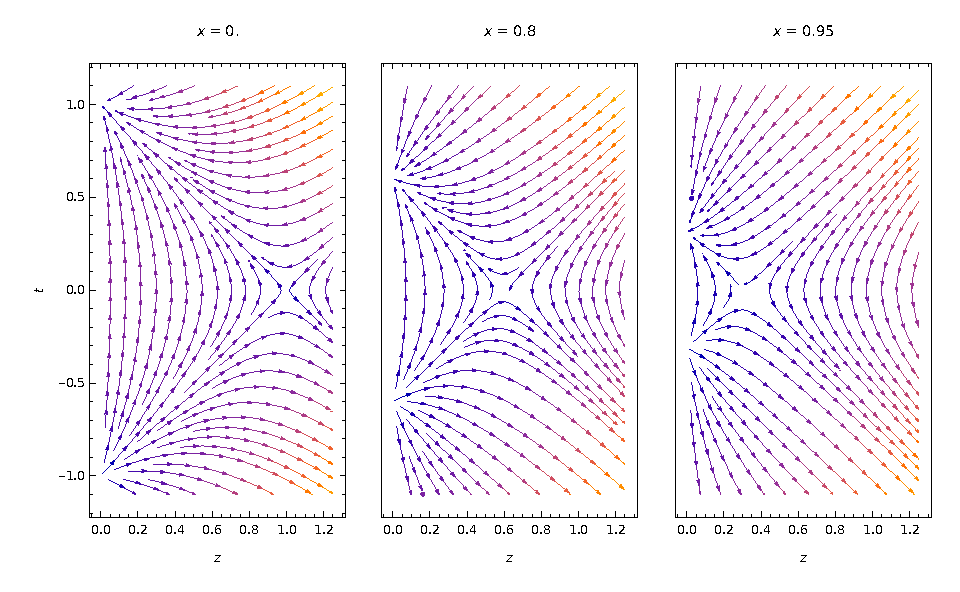
\includegraphics[width=.8\linewidth]{img/modFlowXsection.pdf}
	\hspace{2em}
	\vspace{-2ex}
	\caption{Modular flow at constant $x$ slices}
	\end{figure}
	
	\begin{figure}[!ht]
	\centering
	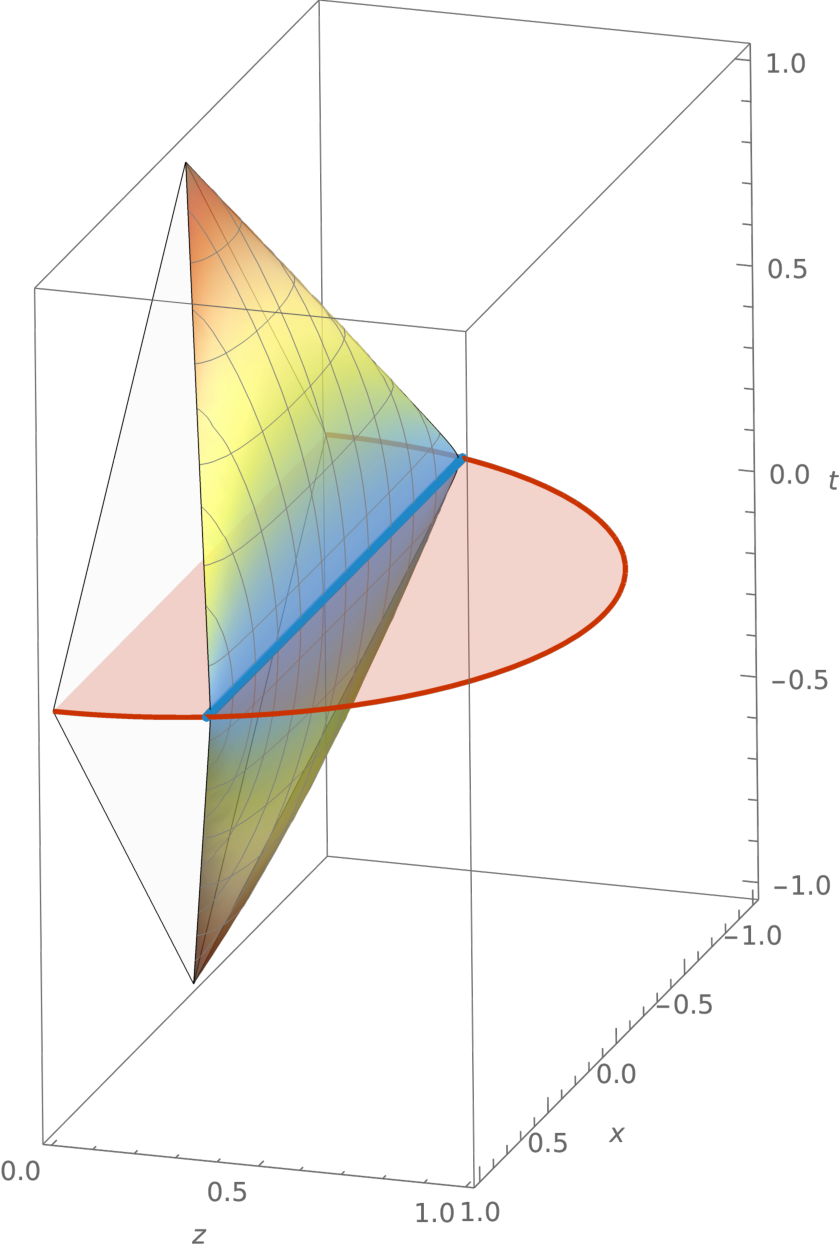
\includegraphics[width=.35\linewidth]{img/modFlowCutoff.pdf}
%	\hspace{2em}
%	\vspace{-2ex}
	\caption{Integral surface of the modular flow starting from $t = 0,\ z = z_c$. Here we've chosen $\frac{L}{2} = 1$ while $z_c = 0.35$.}
	\end{figure}
	
\section{Entropy as Noether Charge}
	Ref: \textcite{Wald:1993nt,Iyer:1994ys,Iyer:1995kg}.
	
	Ref: \textcite{Lewkowycz:2013nqa,Faulkner:2013ana}. 
	
	Gravitational entropy is the Noether charge $Q_\xi$ associated with some horizon generator $\xi$. In the case of entanglement entropy between a simple interval and its complement, we've found its corresponding modular flow in the bulk, which is precisely the horizon generator of the Rindler patch. We then aim to compute the charge variation using the covariant formula:
	\begin{equation}
		\var{Q}_{\xi} [\var{g}, g]
		= \int_{\pd\Sigma}
			\chi_\xi
		= \frac{1}{16 \pi G}
			\int_{\pd\Sigma}
			\sqrt{|g|} \dd{x}^{\alpha}
				\varepsilon_{\alpha\mu\nu}\,
				k_\xi^{\mu\nu} [\var{g}, g]
	\end{equation}
	\begin{equation}
	\begin{aligned}
		k_\xi^{\mu\nu}[\var g, g]
		= \frac{1}{2} \Big \{
		& \xi^{\nu}\nabla^{\mu} \var g^{\alpha}{}_{\alpha}
		- \xi^{\nu} \nabla_{\alpha} \var g^{\alpha\mu}
		+ \xi_{\alpha} \nabla^{\nu} \var g^{\alpha\mu}  \\
		&+ \frac{1}{2} \var g^{\alpha}{}_{\alpha} \nabla^{\nu} \xi^{\mu}
		- \frac{1}{2} \var g^{\nu\alpha} \nabla_{\alpha}\xi^{\mu}
		+ \frac{1}{2} \var g^{\nu\alpha} \nabla^{\mu} \xi_{\alpha} \\
		&- (\mu \leftrightarrow \nu) \Big \}
	\end{aligned}
	\label{kdef}
	\end{equation}
	However, to compute $\var{Q}$ we need to consider a particular metric variation $\var{g}_{\mu\nu}$ in the phase space of solutions. There is no free parameter in Poincar\'e $\mrm{AdS}_3$, unless we turn on temperature; this leads to the BTZ geometry. 
	
	We thus have to repeat the calculations above to get the geodesic $\gamma$ and modular generators $\xi^\mu$ in the new backgrounds. However, it is convenient to remember that all BTZ black holes are locally equivalent to the pure $\mrm{AdS}_3$; we can then map Poincar\'e $(u,v,z)$ to BTZ $(t,r,\phi)$ by \cite{Hubeny:2007xt}:
	\begin{equation}
		u,v = \sqrt{\frac{r^2 - r_+^2}{r^2 - r_-^2}}\,
			e^{(\phi\pm t)\,2T_{u,v}},
	\quad
		z = \sqrt{\frac{r_+^2 - r_-^2}{r^2 - r_-^2}}\,
			e^{\phi r_+ + t r_-},
	\end{equation}
	\begin{gather}
		r_\pm = T_u \pm T_v,
	\quad
		8GM = r_+^2 + r_-^2
		= 2\,(T_u^2 + T_v^2),
	\quad
		4GJ = r_+ r_-
		= T_u^2 - T_v^2,
	\end{gather}
	\begin{equation}
		\dd{s}^2
		= \frac{r^2 \dd{r}^2}{
				(r^2 - r_+^2)
				(r^2 - r_-^2)
			}
			+ T_u^2 \dd{u}^2
			+ T_v^2 \dd{v}^2
			+ (r^2 - T_u^2 - T_v^2) \dd{u} \dd{v}
	\end{equation}
	$\gamma$ and $\xi^\mu$ in BTZ coordinates both follow from this map. 
	
	We now restrict to $t_\pm = 0, \phi_- = -\phi_+$ and set $T_u = T_v = T$ for convenience; in this case the RT surface is given by \cite{Rangamani:2016dms}:
	\begin{equation}
		r(\phi) = \frac{2T\cosh TL}{
				\sqrt{\cosh^2 TL - \cosh^2 2T\phi}
			}
	\end{equation}
	The charge variation has a nice form under the above simplifications; in this case we have $
		\var{Q}_{\xi}
		= \int \dd{\phi} (\chi_\xi)_\phi
	$, where:
	\begin{equation}
		(\chi_\xi)_\phi
		= \frac{\var{T} \coth (LT)}{2G}
			\pqty{
				1 - {\frac{r}{\sqrt{r^2 - 4T^2}}}
				\frac{\cosh (2T\phi)}{\cosh (TL)}
			}
	\end{equation}
	
	The $\int_\gamma \dd{\phi}$ integration can be done at the asymptotic infinity $r\to\infty$ instead, due to Stokes' theorem; this gives the following result:
	\begin{equation}
		\var{Q}_\xi
		= \frac{\var{T}}{2G} \pqty{
				L \coth (LT) - \frac{1}{T}
			}
	\end{equation}
	With a final integration w.r.t.~$\var{T}$ in the phase phase, we recover the resulting charge, which agrees with the entanglement entropy in \cite{Rangamani:2016dms} up to an overall constant shift:
	\begin{equation}
		Q_\xi = \frac{1}{2G} \log \frac{\sinh (LT)}{T}
	\end{equation}
	
\subsection{With constant cutoff}
	Now we consider constant cutoff at $r = r_c$. Again we need to trade $L_\infty$ above with the coordinate length of the interval $L$ at the cutoff $r_c$. The relation can be solved by looking at the geodesic equation, which is slightly non-trivial this time:
	\begin{equation}
		\frac{\cosh (L_\infty T)}{\cosh (LT)}
		= \frac{r_c}{\sqrt{r_c^2 - 4T^2}}
	\end{equation}
	\begin{equation}
		r(\phi) = \frac{2T\cosh TL}{
				\sqrt{\cosh^2 TL - \pqty\big{
					1 - \frac{4T^2}{r_c^2}
				}\cosh^2 2T\phi}
			}
	\end{equation}
	We then compute the charges like before, and we have:
	\begin{equation}
		\var{Q}_\xi
		= \frac{\var{T}}{2G} \pqty{
				L \coth (LT) - \frac{1}{T}
			}
			\frac{1}{\sqrt{
				1 + \frac{4T^2}{r_c^2 \sinh^2 LT}
			}}
	\end{equation}
	
	We haven't found a nice way to compute this integral directly, but we note that the magical square root factor appears again in the $T\to 0$ limit:
	\begin{equation}
		T\to 0,
	\quad
		\sqrt{
			1 + \frac{4T^2}{r_c^2 \sinh^2 LT}
		}
		\to \sqrt{
			1 + \frac{4}{r_c^2 L^2}
		}
		\to \sqrt{
			1 + \frac{4z_c^2}{L^2}
		}
	\end{equation}
	This inspire us to take $L\pdd{L}$ first, and then compute the $\int \var{T}$; this is, surprisingly, doable, and reproduces the $C(L)$ function in \textcite{Lewkowycz:2019xse} in the $T \to 0$ limit:
	\begin{equation}
		L \pdv{L}\,Q_\xi
		= \frac{1}{2G}
			\frac{LT \coth LT}{\sqrt{
				1 + \frac{4T^2}{r_c^2 \sinh^2 LT}
			}}
	\qquad\text{(up to const.)}
	\end{equation}
	
	Note that we have \textit{not} been very careful about the possible $L,T$ dependent integration constants. If we then do the $L$ integration from the above $L \pdv{L}\,Q_\xi$, we then find the charge up to some $L,T$ dependent integration constants:
	\begin{equation}
		Q_\xi
		= \frac{1}{2G} \mop{arctanh}
			\frac{1}{\sqrt{
				1 + \frac{4T^2}{r_c^2 \sinh^2 LT}
			}}
		= \frac{1}{2G} \log
			\frac{
				\sqrt{
					1 + \frac{4T^2}{r_c^2 \sinh^2 LT}
				} + 1
			}{
				\sqrt{
					1 + \frac{4T^2}{r_c^2 \sinh^2 LT}
				} - 1
			}
	\qquad\text{(up to const.)}
	\end{equation}
	
	
	
	
	
	
	
	

\vspace{1.2\baselineskip}
\raggedright
\printbibliography[%
%	title = {参考文献} %
	,heading = bibintoc
]
\end{document}
